\documentclass{article}
\usepackage[utf8]{inputenc}
\usepackage{amsmath}
\usepackage{nicematrix}
\usepackage{graphicx}
\usepackage{amssymb}
\usepackage[left=3cm,right=3cm]{geometry}

\begin{document}
{\scshape } \hfill {\scshape DISCRETE STRUCTURES (CO1007) - Homework 09 - Connectivity} \hfill {\scshape }
\smallskip

\hrule

\begin{table}[h]
\begin{tabular}{|c|c|c|c|}
\hline
\multicolumn{4}{|c|}{\textbf{GROUP 1984 ------ MEMBER LIST}}        \\ \hline
\textbf{No.} & \textbf{Name}        & \textbf{ID} & \textbf{Role} \\ \hline
\textbf{1}   & Quach Dang Giang     & 1952044     & Leader, 25\% (of the current work)  \\ \hline
\textbf{2}   & Huynh Phuoc Thien    & 1952463     & Member, 35\%  \\ \hline
\textbf{3}   & Tran Nguyen Anh Khoa & 1911419     & Member, 40\%  \\ \hline
\end{tabular}
\end{table}
\textbf{The number of mandatory exercise: 23/23}
\section*{Question 1}
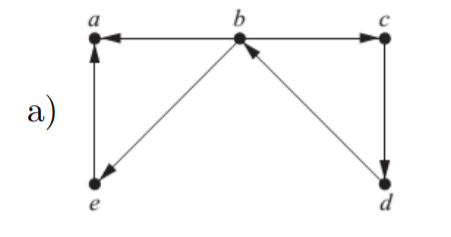
\includegraphics[]{Question 1/connectivity_1.a.png}
\newline
The graph is weakly connected because there is no path from a to any other vertices.
\newline
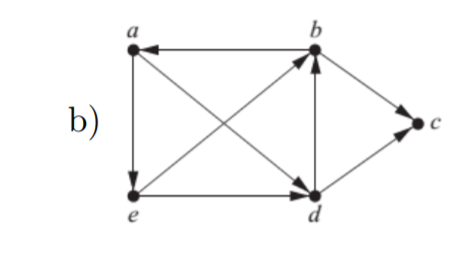
\includegraphics[]{Question 1/connectivity_1.b.png}
\newline
The graph is weakly connected because there is no path from a to any other vertices.
\newline
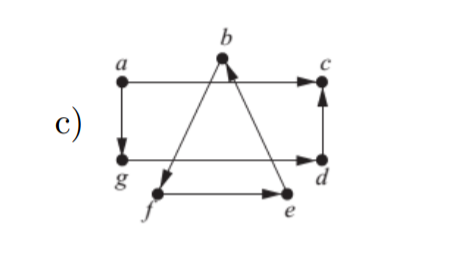
\includegraphics[]{Question 1/connectivity_1.c.png}
\newline
The graph is neither strongly connected nor weakly connected because there is no path from a to b in the underlying undirected graph.
\newline
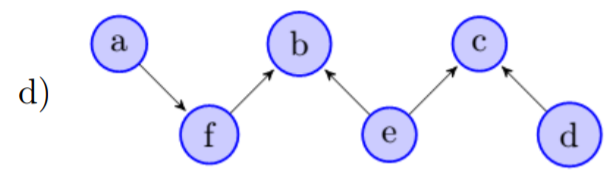
\includegraphics[]{Question 1/connectivity_1.d.png}
\newline
The graph is weakly connected because there is no path from b to any other vertices.
\newline
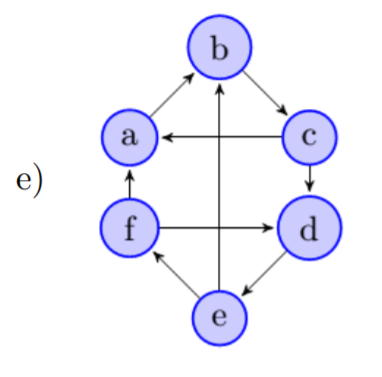
\includegraphics[]{Question 1/connectivity_1.e.png}
\newline
The graph is strongly connected.
\newline

\section*{Question 2}
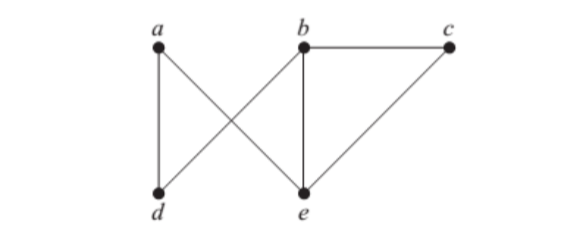
\includegraphics[]{Question 2/connectivity_2.png}
\newline
\textbf{a, e, b, c, b} form a path of length 4, this path is not simple because edge bc is passed 2 times\\
\textbf{c, b, d, a, e, c} form path of length 5, this path is simple and circuit.

\section*{Question 3}
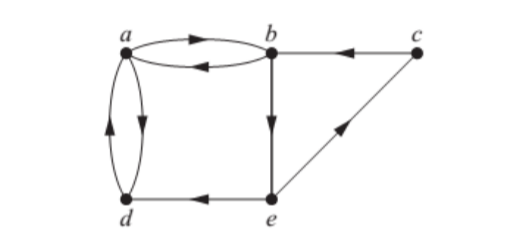
\includegraphics[]{Question 3/connectivity_3.png}
\newline
a, b, e, c, b form a simple path of length 4\\
a, d, a, d, a form a circuit path of length 4

\section*{Question 4}
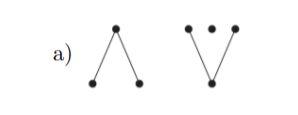
\includegraphics[]{Question 4/connectivity_4.a.png}
\newline
The graph is not a connected graph
\newline
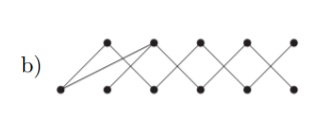
\includegraphics[]{Question 4/connectivity_4.b.png}
\newline
The graph is a connected graph
\newline
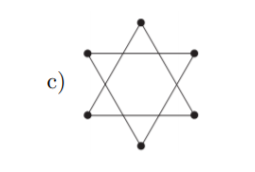
\includegraphics[]{Question 4/connectivity_4.c.png}
\newline
The graph is not a connected graph
\newline

\section*{Question 5}
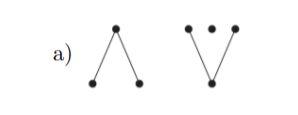
\includegraphics[]{Question 4/connectivity_4.a.png}
\newline
Graph a) has 3 connected components
\newline
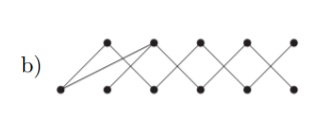
\includegraphics[]{Question 4/connectivity_4.b.png}
\newline
Graph b) has 1 connected component
\newpage
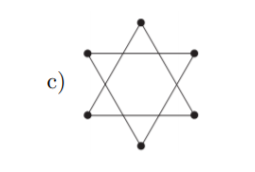
\includegraphics[]{Question 4/connectivity_4.c.png}
\newline
Graph b) has 2 connected components
\newline

\section*{Question 6}
Let the two different vertices be a and b.
\subsection*{a)}
There are two path of length 2\\
\begin{figure}[h]
    \centering
    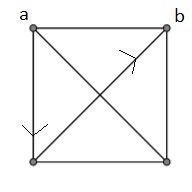
\includegraphics{Question 6/connectivity_6.a.1.png}
    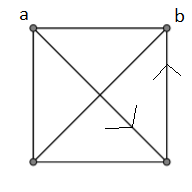
\includegraphics{Question 6/connectivity_6.a.2.png}
\end{figure}
\subsection*{b)}
There are two path of length 3\\
\begin{figure}[h]
    \centering
    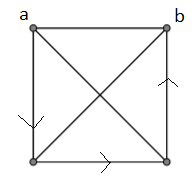
\includegraphics{Question 6/connectivity_6.b.1.png}
    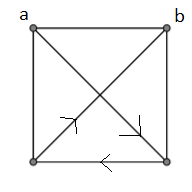
\includegraphics{Question 6/connectivity_6.b.2.png}
\end{figure}

\section*{Question 7}
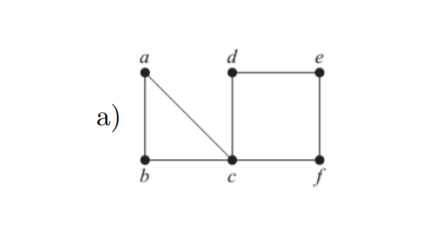
\includegraphics[]{Question 7/connectivity_7.1.png}
\newline
Cut vertex: c
\newline
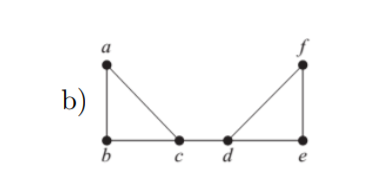
\includegraphics[]{Question 7/connectivity_7.2.png}
\newline
Cut vertex: c, d
\newline
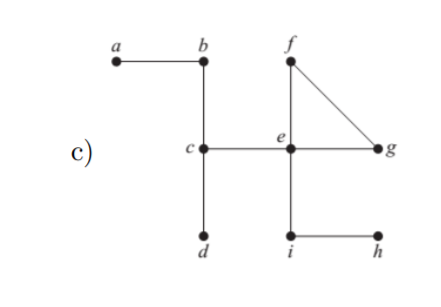
\includegraphics[]{Question 7/connectivity_7.3.png}
\newline
Cut vertex: b, c, e, i

\section*{Question 8}
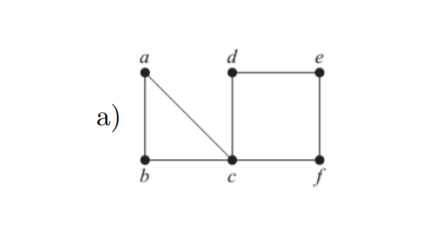
\includegraphics[]{Question 7/connectivity_7.1.png}
\newline
This graph has no cut edge
\newline
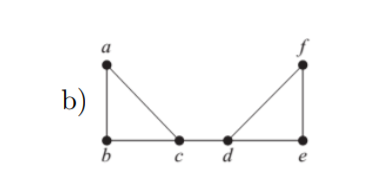
\includegraphics[]{Question 7/connectivity_7.2.png}
\newline
Cut edge: cd
\newline
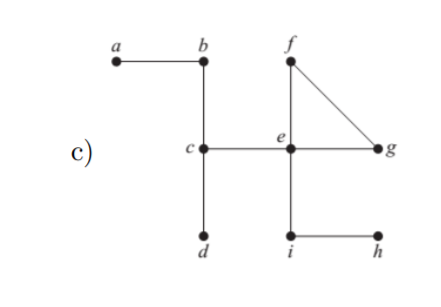
\includegraphics[]{Question 7/connectivity_7.3.png}
\newline
Cut edge: ab, bc, cd, ce, ei, ih

\section*{Question 9}
\subsection*{a)}
$C_n$ has no cut edge because if we remove any edge, the graph still remain a connected component
Example: $C_4$
\newline
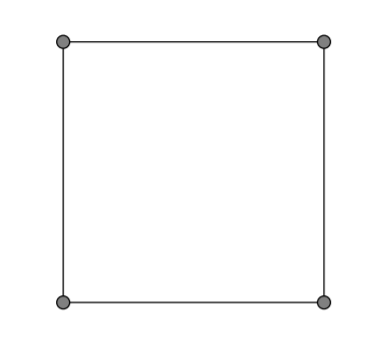
\includegraphics[]{Question 9/connectivity_9.a.png}
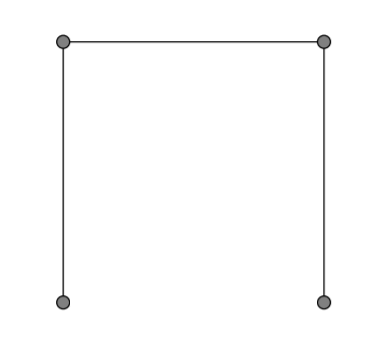
\includegraphics[]{Question 9/connectivity_9.a.edited.png}
\newline
\subsection*{b)}
$K_n$ has no cut edge because if we remove any edge, the graph still remain a connected component
Example: $K_4$
\newline
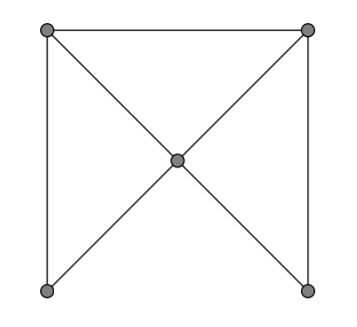
\includegraphics[]{Question 9/connectivity_9.b.edited.png}
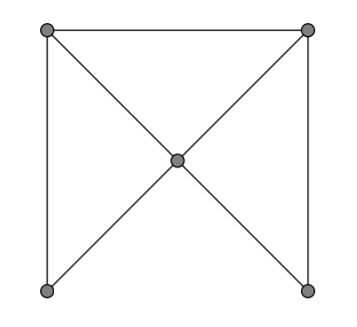
\includegraphics[]{Question 9/connectivity_9.b.edited.png}
\newline
\subsection*{c)}
$K_n$ has no cut edge because if we remove any edge, the graph still remain a connected component
Example: $K_4$
\newline
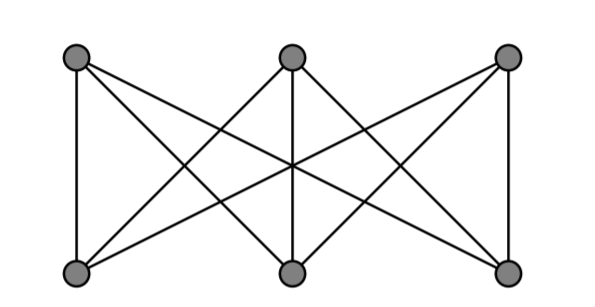
\includegraphics[scale = 0.5]{Question 9/connectivity_9.c.png}
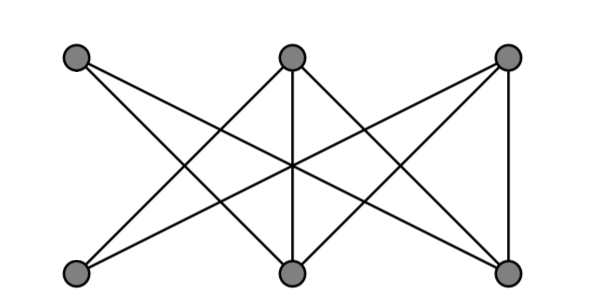
\includegraphics[scale = 0.5]{Question 9/connectivity_9.c.edited.png}
\newline

\section*{Question 10}
\subsection*{a)}
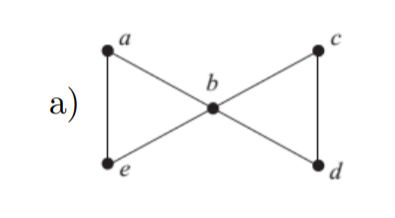
\includegraphics[]{Question 10/connectivity_10.a.png}
\newline
$ \kappa(G) = 1, \lambda(G) = 2 $
\subsection*{b)}
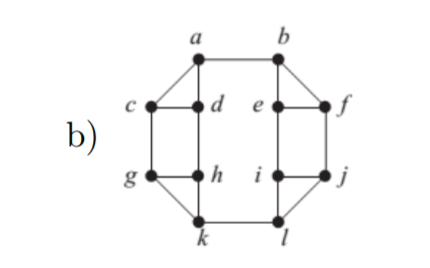
\includegraphics[]{Question 10/connectivity_10.b.png}
\newline
$ \kappa(G) = 2, \lambda(G) = 2 $

\section*{Question 11}
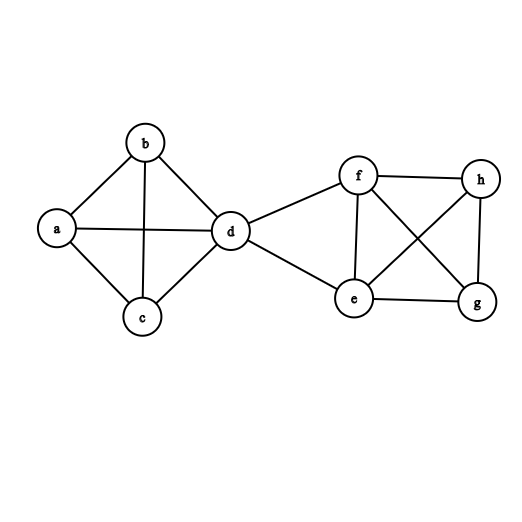
\includegraphics[scale = 0.5]{Question 11/connectivity_11.png}

\section*{Question 12}
An undirected graph has an Euler circuit if all vertex's degree are odd and has an Euler path if every vertex have even degree or exactly two vertex have odd degree.
\newline
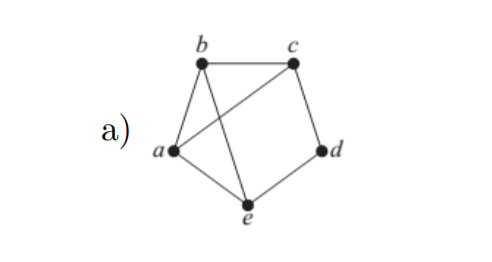
\includegraphics[]{Question 12/connectivity_12.a.png}
\newline
Graph a) has 4 odd degree vertices\\
$\Rightarrow$ Graph a) has no Euler circuit and has no Euler path
\newline
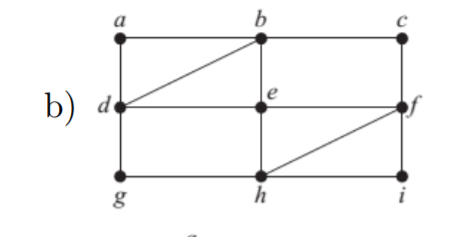
\includegraphics[]{Question 12/connectivity_12.b.png}
\newline
All vertex in graph b) are even degree\\
Graph b) has Euler circuit\\
Path sequence: \{a,b\},\{b,d\},\{d,e\},\{e,f\},\{f,h\},\{h,e\},\{e,b\},\{b,c\},\{b,c\},\{c,f\},\{f,i\},\{i,h\},\{h,g\},\{g,d\},\{d,a\}
\newline
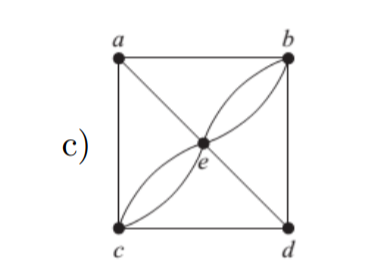
\includegraphics[]{Question 12/connectivity_12.c.png}
\newline
Graph c) has 2 odd degree vertices\\
$\Rightarrow$ Graph c) has no Euler circuit and has an Euler path\\
Path sequence: \{a,b\},\{b,e\},\{e,a\},\{a,c\},\{c,e\},\{e,b\},\{b,d\},\{d,e\},\{e,c\},\{c,d\}
\newline
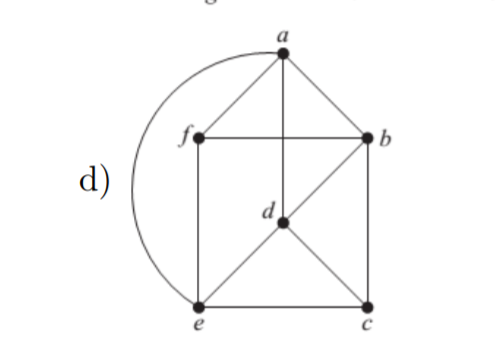
\includegraphics[]{Question 12/connectivity_12.d.png}
\newline
Graph d) has 2 odd degree vertices\\
$\Rightarrow$ Graph d) has no Euler circuit and has an Euler path\\
Path sequence: \{f,a\},\{a,e\},\{e,d\},\{d,b\},\{b,a\},\{a,d\},\{d,c\},\{c,b\},\{b,f\},\{f,e\},\{e,c\}
\newline
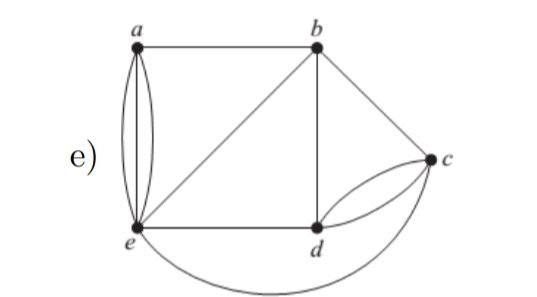
\includegraphics[]{Question 12/connectivity_12.e.png}
\newline
All vertex in graph b) are even degree\\
Graph e) has Euler circuit\\
Path sequence: \{a,b\},\{b,e\},\{e,d\},\{d,b\},\{b,c\},\{c,d\},\{d,c\},\{c,e\},\{e,a\},\{a,e\},\{e,a\}
\newline
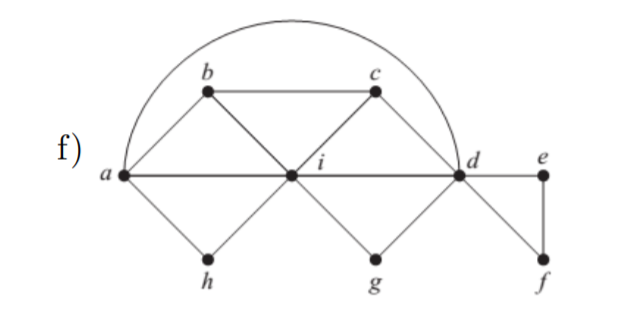
\includegraphics[]{Question 12/connectivity_12.f.png}
\newline
Graph c) has 2 odd degree vertices\\
$\Rightarrow$ Graph c) has no Euler circuit and has an Euler path\\
Path sequence: \{b,a\},\{a,i\},\{i,h\},\{h,a\},\{a,d\},\{d,e\},\{e,f\},\{f,d\},\{d,g\},\{g,i\},\{i,d\},\{d,c\},\{c,i\},\{i,b\},\{b,c\}

\section*{Question 13}
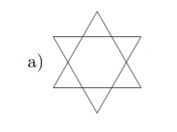
\includegraphics[]{Question 13/connectivity_13.a.png}
\newline
The graph has no odd degree vertex so it contains an Euler circuit.
$\Rightarrow$ The picture shown can be drawn with a pencil in a continuous motion without lifting the pencil or retracing part of the picture.
\newline
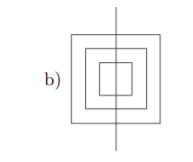
\includegraphics[]{Question 13/connectivity_13.b.png}
\newline
The graph has two odd degree vertices so it contains an Euler path.
$\Rightarrow$ The picture shown can be drawn with a pencil in a continuous motion without lifting the pencil or retracing part of the picture.

\section*{Question 14}
To form an Euler path, the degree of all vertices must be even degree.\\
\subsection*{a)}
The degree of each vertex of $K_n$ has Euler path then $n - 1$. So if $K_n$ has Euler circuit then $n - 1$ must be an even number $\Rightarrow$ $n$ must be an odd number and $n \geqslant 1$.
\subsection*{b)}
For $n \geqslant 3$ (the requirement to form a cycle graph) the degree of every vertices of $C_n$ is 2. So if $C_n$ has Euler circuit then $n \geqslant 3$.
\subsection*{c)}
For $n \geqslant 3$ (the requirement to form a wheel graph) the degree of most vertices of $C_n$ is 3, then it contain odd degree vertex. So $W_n$ has no Euler circuit no matter the value of n.
\subsection*{d)}
The degree of every vertices of $Q_n$ is $n$. So if $K_n$ has Euler circuit then $n$ must be an even number and $n \geqslant 1$.

\section*{Question 15}
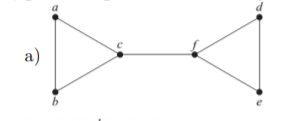
\includegraphics[]{Question 15/connectivity_15.a.png}
\newline
Graph a) has no Hamilton circuit because in the process of finding Hamilton circuit, a new subcircuit is formed.
\newline
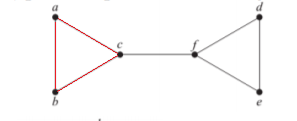
\includegraphics[]{Question 15/connectivity_15.a.edited.png}
\newline
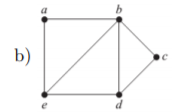
\includegraphics[]{Question 15/connectivity_15.b.png}
\newline
Graph b) has Hamilton circuit.\\
Path sequence: \{a,b\},\{b,e\},\{e,d\},\{d,c\},\{c,a\}
\newline
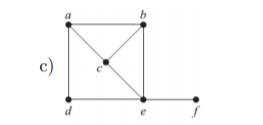
\includegraphics[]{Question 15/connectivity_15.c.png}
\newline
Graph c) has no Hamilton circuit because $deg(f) = 1$.
\newline
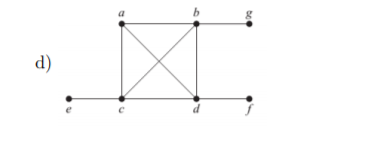
\includegraphics[]{Question 15/connectivity_15.d.png}
\newline
Graph d) has no Hamilton circuit because $deg(e) = deg(f) = deg(g) = 1$.
\newline
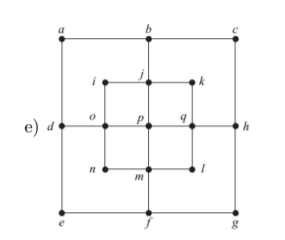
\includegraphics[]{Question 15/connectivity_15.e.png}
\newline
First, we start from vertex a.
\newline
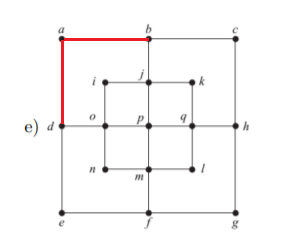
\includegraphics[]{Question 15/connectivity_15.e.4.png}
\newline
From now, if we take the path \{b,j\}:
\newline
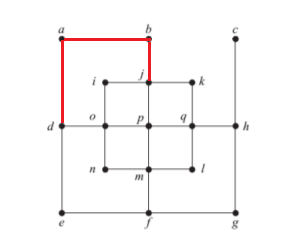
\includegraphics[]{Question 15/connectivity_15.e.3.png}
\newline
Then $deg(c) = 1$, violating with the rule\\
So we have to take the path \{b,c\}, \{c,h\}, \{h,g\}, \{g,f\}
\newline
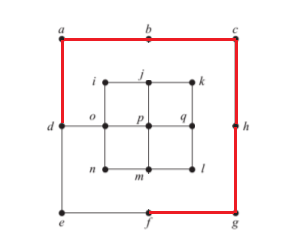
\includegraphics[]{Question 15/connectivity_15.e.1.png}
\newline
From now, if we take the path \{f,e\} then \{e,d\}:
\newline
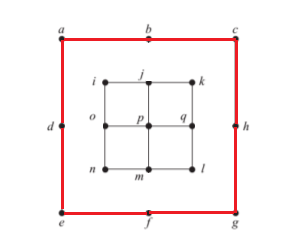
\includegraphics[]{Question 15/connectivity_15.e.2.png}
\newline
A new subcircuit will be formed, violated with the rule so that we can not take this path.\\
We take \{f,m\} instead.
\newline
\includegraphics[]{Question 15/connectivity_15.e.5.png}
\newline
Then $deg(c) = 1$, violating with the rule.\\
\textbf{Conclusion:} The graph has no Hamilton circuit.
\newline
\includegraphics[scale = 2]{Question 15/connectivity_15.f.png}
\newline
First, we start from vertex a.
\newline
\includegraphics[scale = 2]{Question 15/connectivity_15.f.1.png}
\newline
Now, we have two different path, \{b,d\} or \{b,e\}.
\newline
\includegraphics[scale = 2]{Question 15/connectivity_15.f.2.png}
\includegraphics[scale = 2]{Question 15/connectivity_15.f.3.png}
\newline
Both way give us the same result that the paths form a new subcircuit, which violate with the rule.
\textbf{Conclusion:} The graph has no Hamilton circuit.

\section*{Question 16}
\subsection*{a)}
Exist Hamilton circuit in $K_n $for all $ n \geqslant 3 $
\subsection*{b)}
Exist Hamilton circuit in $C_n $for all $ n \geqslant 3 $
\subsection*{c)}
Exist Hamilton circuit in $W_n $for all $ n \geqslant 3 $

\section*{Question 17}
\includegraphics[scale = 1.5]{Question 17/connectivity_17.a.png}
\begin{table}[h]
\begin{tabular}{c|c c c c c c}

  & a & b & c & d & e & z \\ \hline
$\theta$ & 0 & $\infty$ & $\infty$ & $\infty$ & $\infty$ & $\infty$ \\
a & 0 & 2 & 3 & $\infty$ & $\infty$ & $\infty$ \\
b & 0 & 2 & 3 & 7 & 4 & $\infty$ \\
c & 0 & 2 & 3 & 7 & 4 & $\infty$ \\
d & 0 & 2 & 3 & 7 & 4 & 9 \\
e & 0 & 2 & 3 & 5 & 4 & 8 \\
d & 0 & 2 & 3 & 5 & 4 & 7 \\
\end{tabular}
\end{table}
\newline
Path sequence: \{a,b\}, \{b,e\}, \{e,d\}, \{d,z\}
\newline
\includegraphics[scale = 1.7]{Question 17/connectivity_17.a.edited.png}

\includegraphics[scale = 1.5]{Question 17/connectivity_17.b.png}
\begin{table}[h]
\begin{tabular}{c|c c c c c c c c c}

  & a & b & c & d & e & f & g & z \\ \hline
$\theta$ & 0 & $\infty$ & $\infty$ & $\infty$ & $\infty$ & $\infty$ & $\infty$ & $\infty$ \\
a & 0 & 4 & 3 & $\infty$ & $\infty$ & $\infty$ & $\infty$ & $\infty$ \\
b & 0 & 4 & 3 & 9 & $\infty$ & $\infty$ & $\infty$ & $\infty$ \\
c & 0 & 4 & 3 & 6 & 9 & $\infty$ & $\infty$ & $\infty$ \\
d & 0 & 4 & 3 & 6 & 7 & 11 & $\infty$ & $\infty$ \\
e & 0 & 4 & 3 & 6 & 7 & 11 & 12 & $\infty$ \\
f & 0 & 4 & 3 & 6 & 7 & 11 & 12 & 18 \\
g & 0 & 4 & 3 & 6 & 7 & 11 & 12 & 16 \\
\end{tabular}
\end{table}
\newline
Path sequence: \{a,c\},\{c,d\},\{d,e\},\{e,g\},\{g,z\}
\newline
\includegraphics[scale = 1.7]{Question 17/connectivity_17.b.edited.png}

\section*{Question 18}
\includegraphics[]{Question 18/connectivity_18.png}
\newline
There are three possible combination of edge to form a Hamilton path.
\newline
\includegraphics[scale = 0.7]{Question 18/connectivity_18.1.png}
\includegraphics[scale = 0.7]{Question 18/connectivity_18.2.png}
\includegraphics[scale = 0.7]{Question 18/connectivity_18.3.png}
\newline
Because the weight is the same no matter starting point we chose, let's start with a.\\
The path \{a,b\},\{b,c\},\{c,d\},\{d,a\} have the weight of 18\\
The path \{a,b\},\{b,d\},\{d,c\},\{c,a\} have the weight of 19\\
The path \{a,d\},\{d,b\},\{b,c\},\{c,a\} have the weight of 17\\
So the path \{a,d\},\{d,b\},\{b,c\},\{c,a\} have the minimum weight.

\section*{Question 19}
\includegraphics[]{Question 19/connectivity_19.png}
\newline
Using Floyd Warshal algorithm, we have these matrix. The final result is $L^{(8)}$\\
$L^{(0)} = $
$\begin{bmatrix}
0_0 & 8_0 & \infty_0 & 6_0 & \infty_0 & \infty_0 & 7_0 & \infty_0 & \\
3_0 & 0_0 & 2_0 & 1_0 & \infty_0 & \infty_0 & \infty_0 & \infty_0 & \\
\infty_0 & \infty_0 & 0_0 & \infty_0 & 2_0 & 5_0 & \infty_0 & \infty_0 & \\
\infty_0 & \infty_0 & \infty_0 & 0_0 & 4_0 & \infty_0 & 1_0 & \infty_0 & \\
\infty_0 & \infty_0 & \infty_0 & \infty_0 & 0_0 & 9_0 & \infty_0 & 1_0 & \\
\infty_0 & \infty_0 & 4_0 & \infty_0 & \infty_0 & 0_0 & \infty_0 & 3_0 & \\
5_0 & \infty_0 & \infty_0 & \infty_0 & \infty_0 & \infty_0 & 0_0 & 4_0 & \\
\infty_0 & \infty_0 & \infty_0 & \infty_0 & \infty_0 & 7_0 & \infty_0 & 0_0 & \\
\end{bmatrix}$
$L^{(1)} = $
$\begin{bmatrix}
0_0 & 8_0 & \infty_0 & 6_0 & \infty_0 & \infty_0 & 7_0 & \infty_0 & \\
3_0 & 0_0 & 2_0 & 1_0 & \infty_0 & \infty_0 & 10_1 & \infty_0 & \\
\infty_0 & \infty_0 & 0_0 & \infty_0 & 2_0 & 5_0 & \infty_0 & \infty_0 & \\
\infty_0 & \infty_0 & \infty_0 & 0_0 & 4_0 & \infty_0 & 1_0 & \infty_0 & \\
\infty_0 & \infty_0 & \infty_0 & \infty_0 & 0_0 & 9_0 & \infty_0 & 1_0 & \\
\infty_0 & \infty_0 & 4_0 & \infty_0 & \infty_0 & 0_0 & \infty_0 & 3_0 & \\
5_0 & 13_1 & \infty_0 & 11_1 & \infty_0 & \infty_0 & 0_0 & 4_0 & \\
\infty_0 & \infty_0 & \infty_0 & \infty_0 & \infty_0 & 7_0 & \infty_0 & 0_0 & \\
\end{bmatrix}$\\\\\\\\
$L^{(2)} = $
$\begin{bmatrix}
0_0 & 8_0 & 10_2 & 6_0 & \infty_0 & \infty_0 & 7_0 & \infty_0 & \\
3_0 & 0_0 & 2_0 & 1_0 & \infty_0 & \infty_0 & 10_1 & \infty_0 & \\
\infty_0 & \infty_0 & 0_0 & \infty_0 & 2_0 & 5_0 & \infty_0 & \infty_0 & \\
\infty_0 & \infty_0 & \infty_0 & 0_0 & 4_0 & \infty_0 & 1_0 & \infty_0 & \\
\infty_0 & \infty_0 & \infty_0 & \infty_0 & 0_0 & 9_0 & \infty_0 & 1_0 & \\
\infty_0 & \infty_0 & 4_0 & \infty_0 & \infty_0 & 0_0 & \infty_0 & 3_0 & \\
5_0 & 13_1 & 15_2 & 11_1 & \infty_0 & \infty_0 & 0_0 & 4_0 & \\
\infty_0 & \infty_0 & \infty_0 & \infty_0 & \infty_0 & 7_0 & \infty_0 & 0_0 & \\
\end{bmatrix}$
$L^{(3)} = $
$\begin{bmatrix}
0_0 & 8_0 & 10_2 & 6_0 & 12_3 & 15_3 & 7_0 & \infty_0 & \\
3_0 & 0_0 & 2_0 & 1_0 & 4_3 & 7_3 & 10_1 & \infty_0 & \\
\infty_0 & \infty_0 & 0_0 & \infty_0 & 2_0 & 5_0 & \infty_0 & \infty_0 & \\
\infty_0 & \infty_0 & \infty_0 & 0_0 & 4_0 & \infty_0 & 1_0 & \infty_0 & \\
\infty_0 & \infty_0 & \infty_0 & \infty_0 & 0_0 & 9_0 & \infty_0 & 1_0 & \\
\infty_0 & \infty_0 & 4_0 & \infty_0 & 6_3 & 0_0 & \infty_0 & 3_0 & \\
5_0 & 13_1 & 15_2 & 11_1 & 17_3 & 20_3 & 0_0 & 4_0 & \\
\infty_0 & \infty_0 & \infty_0 & \infty_0 & \infty_0 & 7_0 & \infty_0 & 0_0 & \\
\end{bmatrix}$\\\\\\\\
$L^{(4)} = $
$\begin{bmatrix}
0_0 & 8_0 & 10_2 & 6_0 & 10_4 & 15_3 & 7_0 & \infty_0 & \\
3_0 & 0_0 & 2_0 & 1_0 & 4_3 & 7_3 & 2_4 & \infty_0 & \\
\infty_0 & \infty_0 & 0_0 & \infty_0 & 2_0 & 5_0 & \infty_0 & \infty_0 & \\
\infty_0 & \infty_0 & \infty_0 & 0_0 & 4_0 & \infty_0 & 1_0 & \infty_0 & \\
\infty_0 & \infty_0 & \infty_0 & \infty_0 & 0_0 & 9_0 & \infty_0 & 1_0 & \\
\infty_0 & \infty_0 & 4_0 & \infty_0 & 6_3 & 0_0 & \infty_0 & 3_0 & \\
5_0 & 13_1 & 15_2 & 11_1 & 15_4 & 20_3 & 0_0 & 4_0 & \\
\infty_0 & \infty_0 & \infty_0 & \infty_0 & \infty_0 & 7_0 & \infty_0 & 0_0 & \\
\end{bmatrix}$
$L^{(5)} = $
$\begin{bmatrix}
0_0 & 8_0 & 10_2 & 6_0 & 10_4 & 15_3 & 7_0 & 11_5 & \\
3_0 & 0_0 & 2_0 & 1_0 & 4_3 & 7_3 & 2_4 & 5_5 & \\
\infty_0 & \infty_0 & 0_0 & \infty_0 & 2_0 & 5_0 & \infty_0 & 3_5 & \\
\infty_0 & \infty_0 & \infty_0 & 0_0 & 4_0 & 13_5 & 1_0 & 5_5 & \\
\infty_0 & \infty_0 & \infty_0 & \infty_0 & 0_0 & 9_0 & \infty_0 & 1_0 & \\
\infty_0 & \infty_0 & 4_0 & \infty_0 & 6_3 & 0_0 & \infty_0 & 3_0 & \\
5_0 & 13_1 & 15_2 & 11_1 & 15_4 & 20_3 & 0_0 & 4_0 & \\
\infty_0 & \infty_0 & \infty_0 & \infty_0 & \infty_0 & 7_0 & \infty_0 & 0_0 & \\
\end{bmatrix}$\\\\\\\\
$L^{(6)} = $
$\begin{bmatrix}
0_0 & 8_0 & 10_2 & 6_0 & 10_4 & 15_3 & 7_0 & 11_5 & \\
3_0 & 0_0 & 2_0 & 1_0 & 4_3 & 7_3 & 2_4 & 5_5 & \\
\infty_0 & \infty_0 & 0_0 & \infty_0 & 2_0 & 5_0 & \infty_0 & 3_5 & \\
\infty_0 & \infty_0 & 17_6 & 0_0 & 4_0 & 13_5 & 1_0 & 5_5 & \\
\infty_0 & \infty_0 & 13_6 & \infty_0 & 0_0 & 9_0 & \infty_0 & 1_0 & \\
\infty_0 & \infty_0 & 4_0 & \infty_0 & 6_3 & 0_0 & \infty_0 & 3_0 & \\
5_0 & 13_1 & 15_2 & 11_1 & 15_4 & 20_3 & 0_0 & 4_0 & \\
\infty_0 & \infty_0 & 11_6 & \infty_0 & 13_6 & 7_0 & \infty_0 & 0_0 & \\
\end{bmatrix}$
$L^{(7)} = $
$\begin{bmatrix}
0_0 & 8_0 & 10_2 & 6_0 & 10_4 & 15_3 & 7_0 & 11_5 & \\
3_0 & 0_0 & 2_0 & 1_0 & 4_3 & 7_3 & 2_4 & 5_5 & \\
\infty_0 & \infty_0 & 0_0 & \infty_0 & 2_0 & 5_0 & \infty_0 & 3_5 & \\
6_7 & 14_7 & 16_7 & 0_0 & 4_0 & 13_5 & 1_0 & 5_5 & \\
\infty_0 & \infty_0 & 13_6 & \infty_0 & 0_0 & 9_0 & \infty_0 & 1_0 & \\
\infty_0 & \infty_0 & 4_0 & \infty_0 & 6_3 & 0_0 & \infty_0 & 3_0 & \\
5_0 & 13_1 & 15_2 & 11_1 & 15_4 & 20_3 & 0_0 & 4_0 & \\
\infty_0 & \infty_0 & 11_6 & \infty_0 & 13_6 & 7_0 & \infty_0 & 0_0 & \\
\end{bmatrix}$\\\\\\\\
$L^{(8)} = $
$\begin{bmatrix}
0_0 & 8_0 & 10_2 & 6_0 & 10_4 & 15_3 & 7_0 & 11_5 & \\
3_0 & 0_0 & 2_0 & 1_0 & 4_3 & 7_3 & 2_4 & 5_5 & \\
\infty_0 & \infty_0 & 0_0 & \infty_0 & 2_0 & 5_0 & \infty_0 & 3_5 & \\
6_7 & 14_7 & 16_7 & 0_0 & 4_0 & 12_8 & 1_0 & 5_5 & \\
\infty_0 & \infty_0 & 12_8 & \infty_0 & 0_0 & 8_8 & \infty_0 & 1_0 & \\
\infty_0 & \infty_0 & 4_0 & \infty_0 & 6_3 & 0_0 & \infty_0 & 3_0 & \\
5_0 & 13_1 & 15_2 & 11_1 & 15_4 & 11_8 & 0_0 & 4_0 & \\
\infty_0 & \infty_0 & 11_6 & \infty_0 & 13_6 & 7_0 & \infty_0 & 0_0 & \\
\end{bmatrix}$

\subsection*{Question 20}
\includegraphics[]{Question 20/connectivity_20.a.png}
\includegraphics[]{Question 20/connectivity_20.a.edited.png}
\newline
\includegraphics[]{Question 20/connectivity_20.b.png}
\includegraphics[]{Question 20/connectivity_20.b.edited.png}
\newline
\includegraphics[]{Question 20/connectivity_20.c.png}
\includegraphics[]{Question 20/connectivity_20.c.edited.png}
\newline

\subsection*{Question 21}
\includegraphics[]{Question 21/connectivity_21.a.png}
\newline
Graph a) is $K_{3,3}$. Base on Kuratowski’s theorem, the graph is nonplanar.
\newline
\includegraphics[]{Question 21/connectivity_21.b.png}
\newline
Graph b) is planar, so it can be draw again in order to have no pair of cross edges.
\newline
\includegraphics[]{Question 21/connectivity_21.b.edited.png}
\newline

\subsection*{Question 22}
\includegraphics[]{Question 22/connectivity_22.a.png}
\newline
The dual graph of map a):
\newline
\includegraphics[]{Question 22/connectivity_22.a.graph.png}
\newline
At least 4 colors needed.
\newline
\includegraphics[]{Question 22/connectivity_22.b.png}
\newline
The dual graph of map b):
\newline
\includegraphics[]{Question 22/connectivity_22.b.graph.png}
\newline
At least 2 colors needed.

\subsection*{Question 23}
If n is odd number, the chromatic number is 4 since the vertices of cycle can be given three color and the center vertex is given fourth color.\\
Example: $W_5$
\newline
\includegraphics[]{Question 23/connectivity_23.a.png}
\newline
If n is odd number, the chromatic number is 4 since the vertices of cycle can be given three color and the center vertex is given fourth color.\\
Example: $W_4$
\newline
\includegraphics[]{Question 23/connectivity_23.b.png}
\newline
\end{document}
